\chapter{Related work}\label{chap:comparison}

\begin{figure}[h!]
\centering
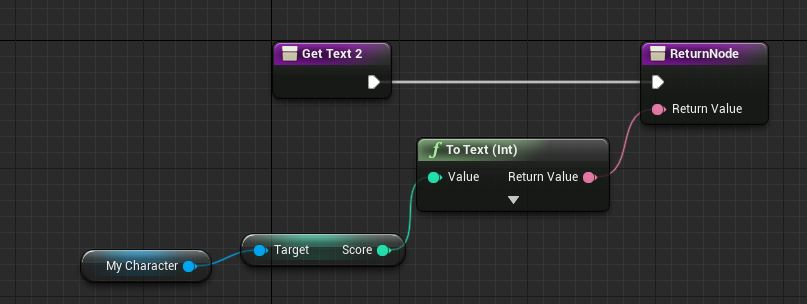
\includegraphics[width=0.9\textwidth]{blueprint}
\caption{Blueprints Visual Scripting\footnote{Screenshot from  \url{https://docs.unrealengine.com/latest/images/Engine/Blueprints/HowTo/BPHT_6/GetScore.jpg}}}
\label{fig:blueprint}
\end{figure}

comparisons

vs Unreal: // very static and cumbersome
    first-class functions
    first-class macros
    substitution
    
    in 4.9.2 no sorting function implemented
        and it's a commercial product
        
        one of the possible areas where a visual language would be handy for anyone, regardless of programming experience is rapid prototyping
        
        if it's static like Blueprint this advantage is greatly diminished
    w/o first-class functions the more cumbersome to implement
    

General desirable characteristics of a scripting language:
	dynamic
	flexible
	suitable for rapid prototyping
	library of basic functions
	complementary to a non-scripting language
	
Unreal Engine
	nope
	static
	rigid
	no sort
	
	does not really complement C++, which is also static and rigid